\documentclass[a4paper,12pt]{article}
\usepackage[swedish]{babel}
\usepackage[utf8]{inputenc}
\usepackage{amsmath, amsthm, amssymb}
\usepackage{graphicx}
\usepackage{enumitem}
\usepackage[a4paper,includeheadfoot,margin=2.54cm]{geometry}
\usepackage{fancyhdr}
\pagestyle{fancy}
\fancyhead[R]{Zacharias Brohn - 9907174297}
\renewcommand{\headrulewidth}{0pt}
\setlength{\headheight}{14.5pt}
%
\begin{document}
%
\section{Dugga 6 - Fråga 7}
Låt $V = \{a, b, c, d, e, f\}$.
\begin{enumerate}[label=\alph*)]
    \item Hur många oriktade grafer $G = (V,E)$ med fyra kanter finns det?
    \item Hur många riktade grafer $G = (V,E)$ med fyra kanter finns det?
\end{enumerate}
%
\section*{Lösning}
%
\begin{enumerate}[label=\alph*)]
    \item För oriktade grafer börjar vi med att räkna antalet möjliga loopar,
    en per nod
    \begin{align}
        \text{Loopar} = 6
    \end{align}
    sedan räknar vi övriga möjliga kanter mellan olika noder, vi har 6 noder
    att välja mellan och vi ska välja 2 av dem eftersom en kant är mellan två
    noder
    \begin{align}
        \binom{6}{2} = 15
    \end{align}
    sedan adderar vi ihop antalet loopar och antalet övriga kanter för att få
    det totala antalet möjliga kanter
    \begin{align}
        6 + 15 = 21
    \end{align}
    och till sist kan vi räkna antalet sätt att välja 4 kanter från det totala
    antalet möjliga kanter
    \begin{align}
        \binom{21}{4} = \frac{21 \cdot 20 \cdot 19 \cdot 18}{4 \cdot 3 \cdot 2 \cdot 1} = 5985
    \end{align}
    \textbf{Svar:} Det finns totalt $5985$ oriktade grafer med fyra
    kanter.
    \item För riktade har vi redan antalet möjliga loopar från föregående
    deluppgift
    \begin{align}
        \text{Loopar} = 6
    \end{align}
    och vi fortsätter som föregående deluppgift med att räkna övriga möjliga
    riktade kanter mellan olika noder, det finns 5 riktningar att välja mellan
    för varje nod, så det blir
    \begin{align}
        6 \cdot 5 = 30
    \end{align}
    sedan adderar vi ihop antalet loopar och antalet övriga kanter igen
    \begin{align}
        6 + 30 = 36
    \end{align}
    då får vi alltså att antalet riktade grafer med fyra kanter är
    \begin{align}
        \binom{36}{4} = \frac{36 \cdot 35 \cdot 34 \cdot 33}{4 \cdot 3 \cdot 2 \cdot 1} = 58905
    \end{align}
    \textbf{Svar:} Det finns totalt $58905$ riktade grafer med fyra kanter.
\end{enumerate}
%
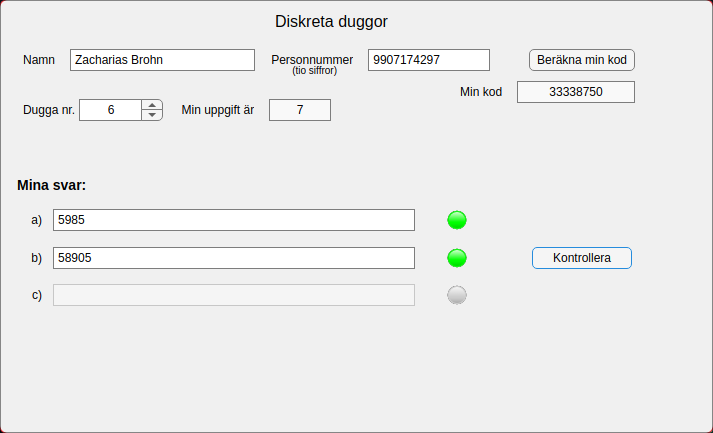
\includegraphics[width=\textwidth]{BheKqYv.png}
%
\end{document}
